\section{B-splines}
\label{sec:FEM Bsplines d=1}

The idea behind B-splines is for the basis element $\varphi_i$ is to be a spline: piece-wise polynomial in each $(x_{k}, x_{k+1})$, with $C^p$-glueing, and the smallest support possible.

\subsubsection{The B-spline basis} Let $t_0 < t_{1} < \cdots < t_m$ be a sequence of points.
Let us construct new points $x_k$ with $k \in \mathbb Z$.
Let us define them by the Cox–de Boor recursion formula
\begin{subequations}
    \label{eq:B-spline}
    \begin{align}
        B_{i,0} (y) & = \begin{dcases}
                            1 & \text{if } y \in [y_i, y_{i+1}) \\
                            0 & \text{otherwise},
                        \end{dcases}
        \\
        B_{i,p} (y) & = \begin{dcases}
                            \frac{y-y_i}{y_{i+p} - y_i} B_{i,p-1}(y) + \frac{y_{i+p+1}-y}{y_{i+p+1} - y_{i+1}} B_{i+1,p-1}(y)
                              & \text{if } y \in [y_i, y_{i+p+1}) \\
                            0 & \text{otherwise}.
                        \end{dcases}
    \end{align}
\end{subequations}
With this additional construction we have that $B_{i,p} \in C^{p-1} (\mathbb R)$.
Their key property is that
\begin{equation*}
    \sum_{i=0}^{m-p-1} B_{i,p}(t) = 1
\end{equation*}
for all $t \in [t_0,t_m]$.
We build the interpolant
\begin{equation*}
    S_p (x) = \sum_j c_{j,p} B_{j,p}(x).
\end{equation*}
For order $p > 1$ we do not have a nice close formula for the interpolation and typical estimates rely on least-square optimisation.

\subsubsection{Linear B-splines}
Let us take a mesh $x_0, \cdots, x_n$ and take $t_i = x_i$ coincides with the piece-wise linear interpolation where $\varphi_i = B_{i-1,1}$.

\subsubsection{Quadratic B-splines}

\paragraph{The finite element} Because of the structure is natural to pick the reference element $K = (-1,1)$.
We can build the B-spline $B_{1,2}$ corresponding to $t_0 = -2, t_1=0, t_2=2$.
Then we have that
\begin{align*}
    \psi_1(y) & = \frac 1 8 ( 1- 2y + y^2)   \\
    \psi_2(y) & = \frac 1 4 ( 3 - y^2 )      \\
    \psi_3(y) & = \frac 1 8 ( 1 + 2y + y^2).
\end{align*}
\begin{figure}[H]
    \centering
    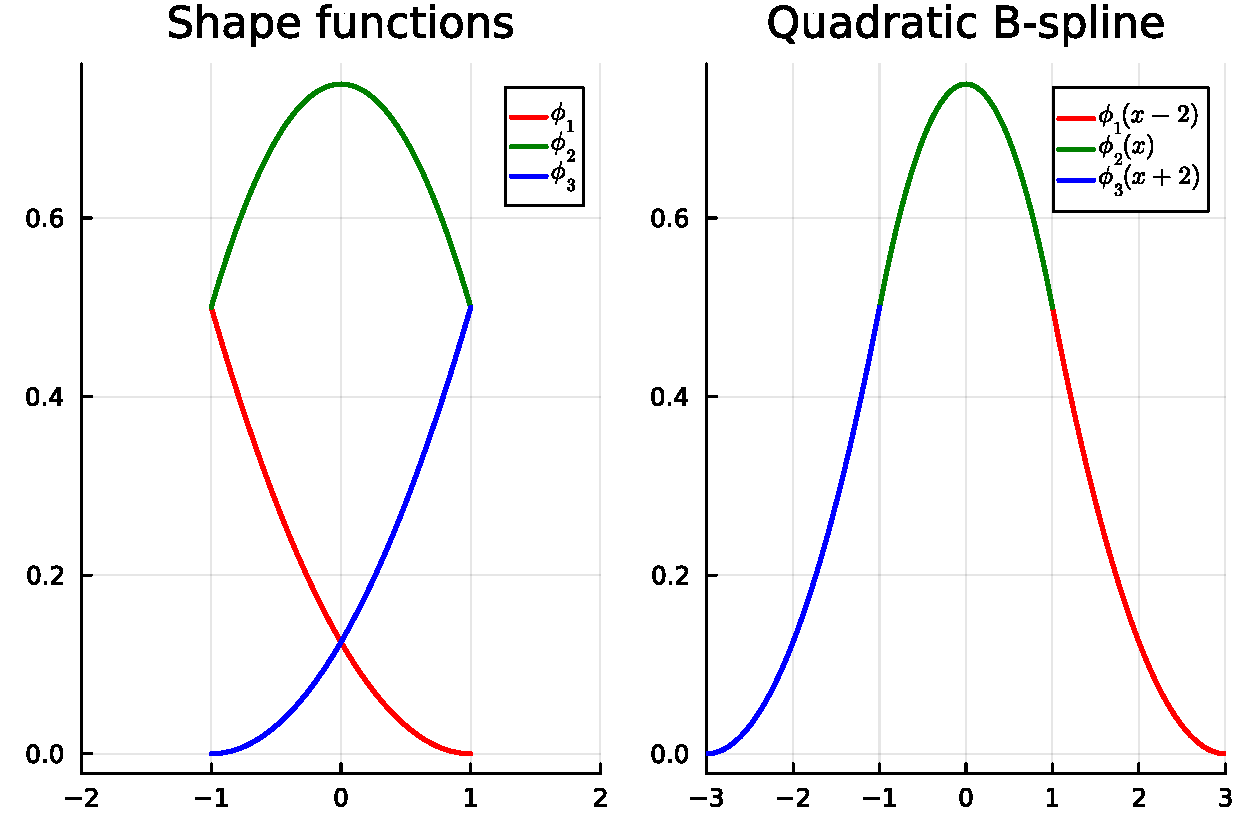
\includegraphics[width=0.5\textwidth]{Bsplines_quadratic_shape.pdf}
    \caption{Quadratic B-spline element}
    \label{fig:FEM d=1 B-spline quadratic}
\end{figure}
We will not discuss the nodal functions $\mathcal N$.

\paragraph{Finite-elements space }
Since we have $C^1$ pasting, given a sub-division $\mathcal T$ of an interval $(a,b)$
by finite-elements space of quadratic B-splines people usually refer to $\mathcal P_{\mathcal T} \cap C^1([a,b])$.

\paragraph{Basis of the finite-elements space on a uniform meshs}
Another approach to constructing B-splines without meshes is to define $b^0(x)$ the characteristic of $[0,1]$ and
\begin{equation*}
    b_p(x) = \int_{x-1}^x b_{p-1}(s) ds.
\end{equation*}
The support of $b_p$ is $(0,p+1)$.
Then, the B-splines on the grid $x_i = i h$ are precisely $b_{p,i,h}(x) = b_p (\frac{x-x_i}{h})$.
\begin{equation*}
    \mathcal P_{\mathcal T}\cap C^1 (a,b) = \left\{ \sum_{i\in \mathbb Z} c_i b_p (\tfrac{x}{h} - i) : c_i \in \mathbb Z \right\}.
\end{equation*}
Notice that, due to the compact support, this is space is finite-dimensional.

\paragraph{Finite-elements space}
If we take the sub-division $\mathcal T$ corresponding to $x_0 = a, \cdots, x_N = b$,
The basis is given precisely adding enough fictious points
\begin{figure}[H]
    \centering
    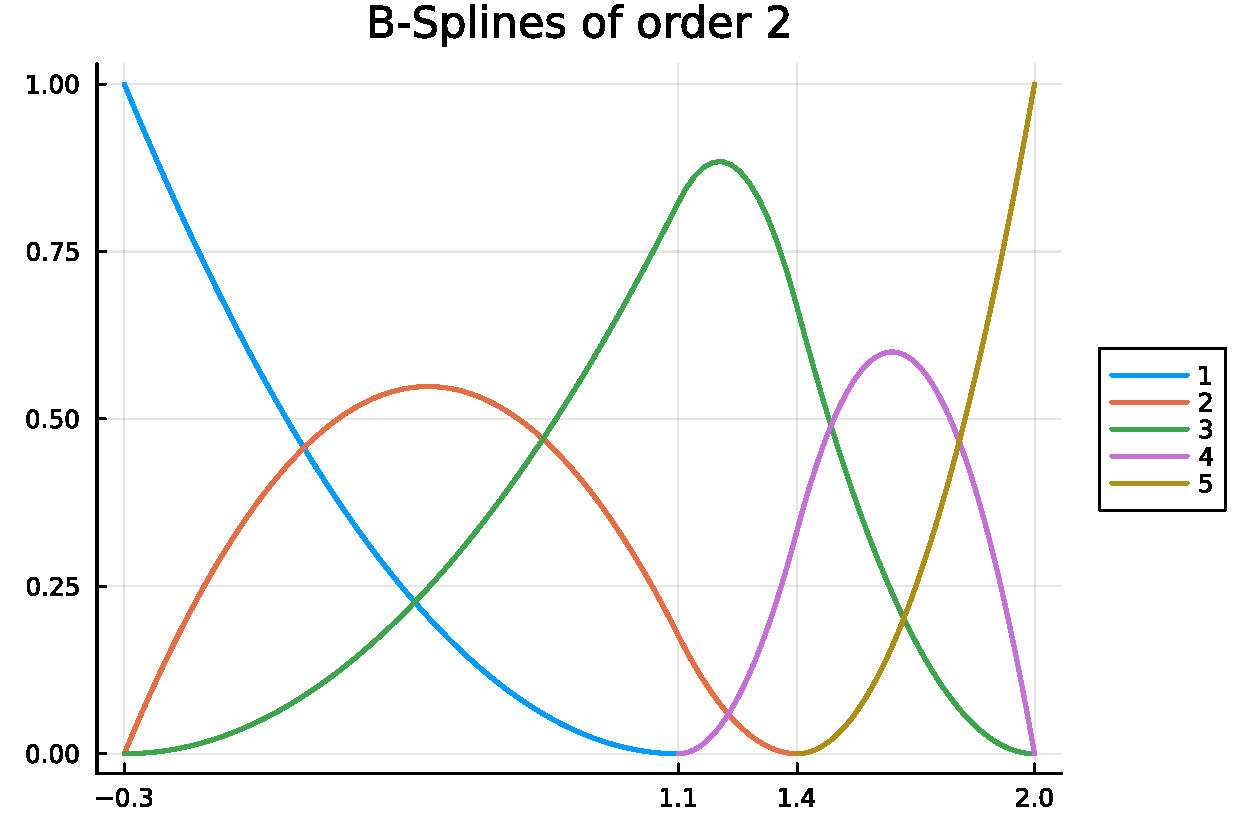
\includegraphics[width=0.5\textwidth]{Bsplines_quadratic_basis}
    \caption{B-splines of order 2 with $x_0 = -0.3, x_1 = 1.1, x_2=1.4, x_3 = 2.0$.}
    \label{fig:Bspline quadratic basis}
\end{figure}



\subsubsection{Cubic B-splines}
We can follow a similar procedure to obtain the cubic B-splines given, for example, in \Cref{fig:Bspline cubic basis}.
The nodal basis are recovered from the B-spline of points
$t_0 = -3, t_2 = -1, t_1 = -1, t_2 = 2$.
The nodal basis
$\psi_1, \cdots, \psi_4$ are given by
\begin{align*}
    \psi_1 & = \frac 1 {48} (-x^3 + 3x^2 - 3x + 1)   \\
    \psi_2 & = \frac 1 {48} (3x^3 - 3x^2 - 15x + 23) \\
    \psi_3 & = \frac 1 {48} (-3x^3 -3x^2 + 15x + 23) \\
    \psi_4 & = \frac 1 {48} (x^3 + 3x^2 + 3x+1).
\end{align*}
Again, we will not discuss the nodal functions in $\mathcal N$.

\paragraph{Finite-elements space}
When discussing cubic B-splines basis people usually refer to the space $\mathcal P_{\mathcal T} \cap C^2([a,b])$. An example of basis for this space is giving in \Cref{fig:Bspline cubic basis}.
\begin{figure}[H]
    \centering
    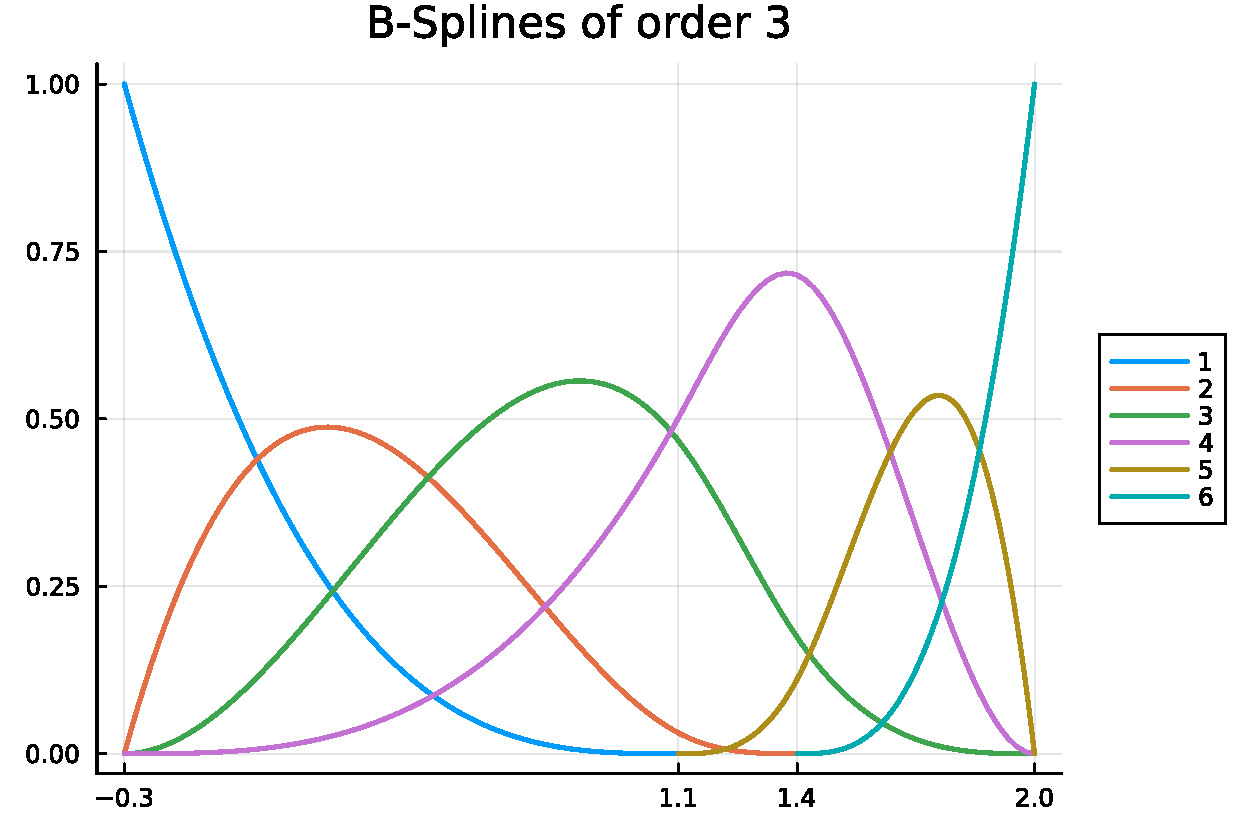
\includegraphics[width=0.5\textwidth]{Bsplines_cubic_basis}
    \caption{B-splines of order 3 with $x_0 = -0.3, x_1 = 1.1, x_2=1.4, x_3 = 2.0$.}
    \label{fig:Bspline cubic basis}
\end{figure}